\chapter{Resultados} \label{chap:resultados}
En la Figura~\ref{fig:CinematicaDirecta} se presentan los resultados obtenidos mediante la simulación en MATLAB de la cinemática directa del robot. La subfigura (a) muestra la configuración espacial del robot en un instante determinado, con la representación de sus articulaciones y eslabones en un entorno tridimensional. Esto permitió verificar visualmente que las posiciones alcanzadas por el efector final corresponden con los valores calculados a partir de los ángulos articulares.

La subfigura (b) muestra un conjunto de gráficas correspondientes a la evolución temporal de diversas variables cinemáticas. Se observa la trayectoria del efector final en los ejes $X$, $Y$ y $Z$, así como sus velocidades y aceleraciones lineales. También se incluyen las gráficas de orientación (ángulos de Euler), velocidades angulares y aceleraciones angulares, las cuales son consistentes con un movimiento continuo y sin cambios bruscos.

Además, se realizó la simulación en los entornos \textit{Gazebo} y \textit{RViz}, donde se implementó el modelo del robot y se le aplicó la trayectoria previamente calculada. En ambos entornos se observó un comportamiento correcto: el robot sigue la trayectoria deseada sin colisiones ni movimientos erráticos. Esto valida la precisión del modelo cinemático directo y la correcta implementación de los ángulos de las juntas. La correspondencia entre los resultados visuales y los obtenidos en las gráficas refuerza la confiabilidad de la simulación realizada.

\begin{figure}[H]
	\centering
	\begin{minipage}[t]{0.49\textwidth}
		\centering
		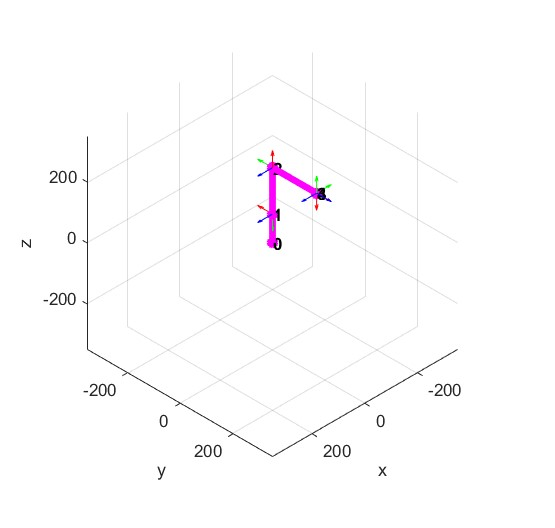
\includegraphics[width=\linewidth]{NuestroRobot_Directa.jpg}
		\caption*{(a) Configuración de juntas del robot}
	\end{minipage}
	\hfill
	\begin{minipage}[t]{0.49\textwidth}
		\centering
		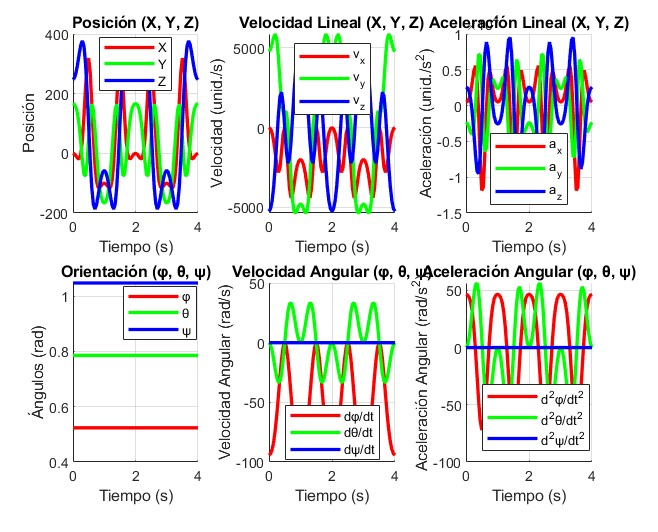
\includegraphics[width=\linewidth]{NuestroRobot_DirectaResultados.jpg}
		\caption*{(b) Resultados de la cinemática directa}
	\end{minipage}
	\caption{Cinemática directa del robot: configuración de juntas y resultados}
	\label{fig:CinematicaDirecta}
\end{figure}

En la Figura~\ref{fig:simulacion_gazebo} se observa al robot modelado en el entorno \textit{Gazebo}, donde se lleva a cabo una simulación física que incluye efectos como la gravedad, colisiones y dinámica. Esta simulación permitió verificar que el robot sigue correctamente la trayectoria establecida, sin desviaciones, oscilaciones anómalas ni interferencias con el entorno.

\begin{figure}[H]
	\centering
	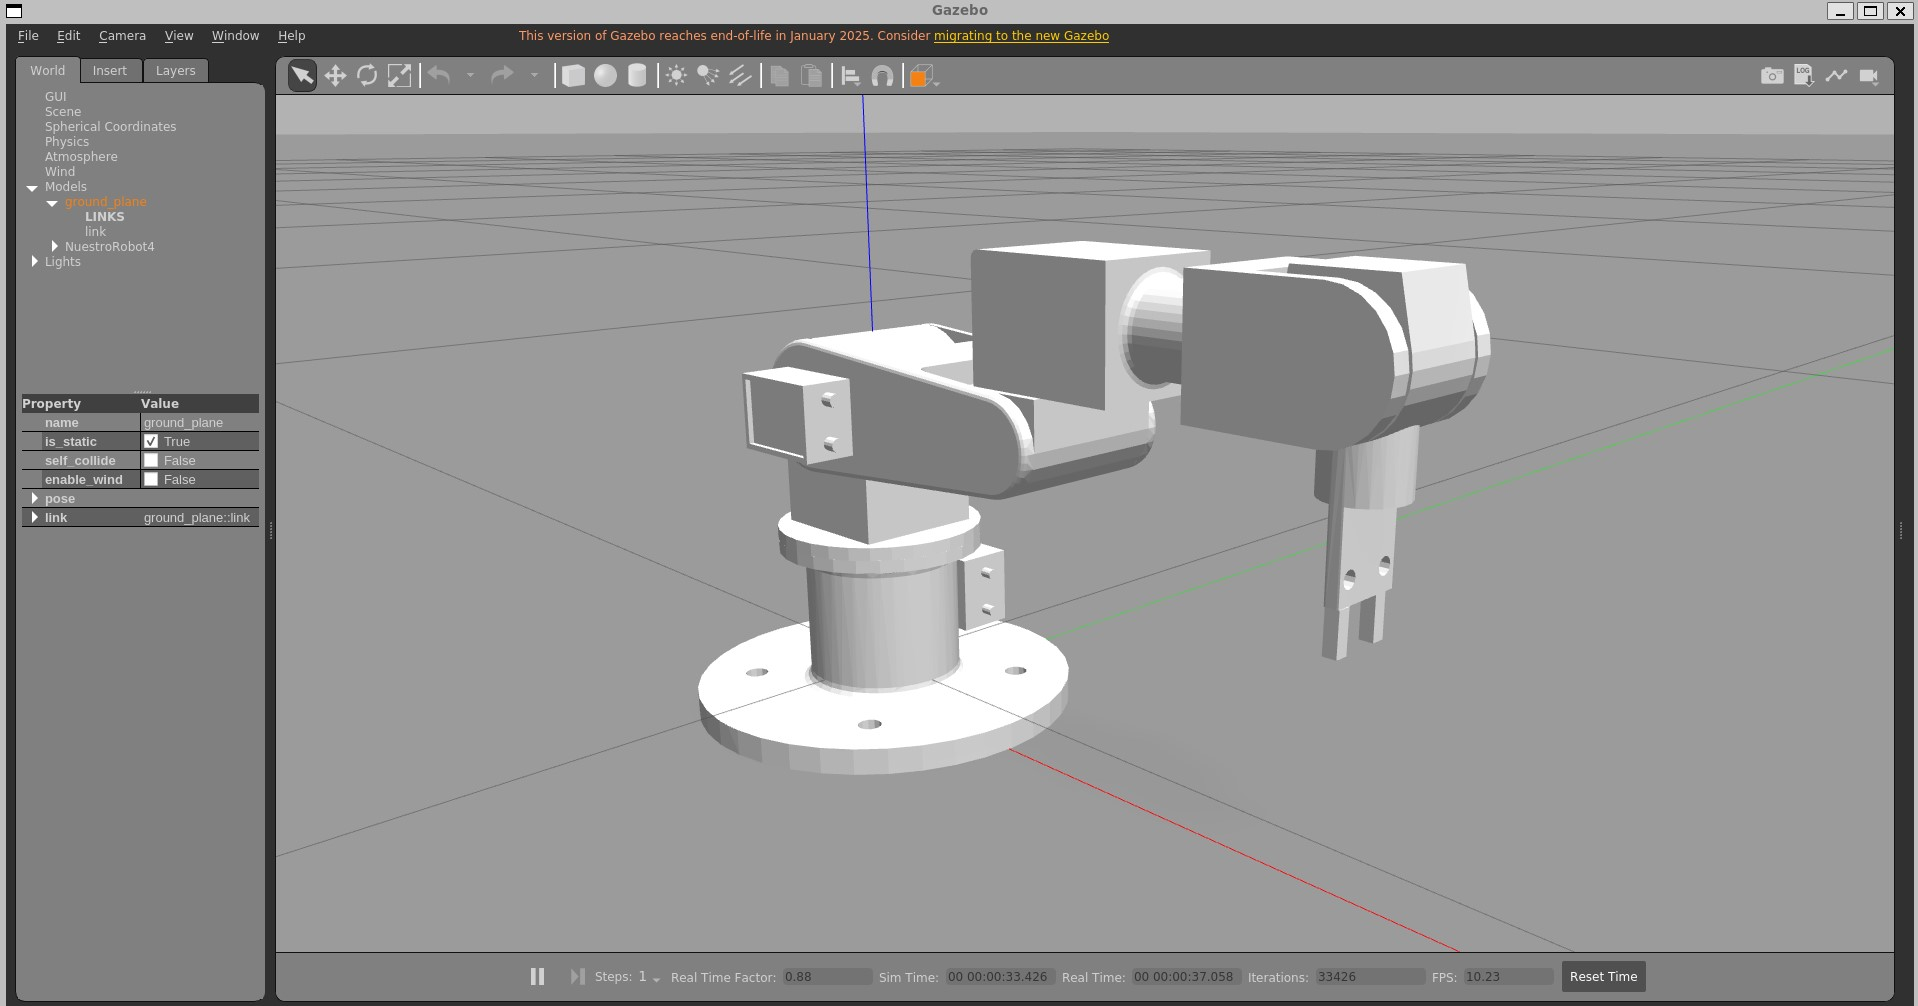
\includegraphics[width=0.8\textwidth]{Gazebo.jpg}
	\caption{Simulación del robot en el entorno Gazebo}
	\label{fig:simulacion_gazebo}
\end{figure}

En la Figura ~\ref{fig:GazeboYrviz} se presenta una vista combinada del robot en \textit{Gazebo} y \textit{RViz}. Mientras que Gazebo ejecuta la física de la simulación, RViz permite la visualización en tiempo real de los datos publicados por los nodos ROS, incluyendo la cinemática del robot y la trayectoria del efector final. En esta visualización, se confirma que el modelo de RViz reproduce de manera precisa los movimientos generados en Gazebo, lo cual indica que la cinemática directa y la publicación de transformaciones se implementaron correctamente.

Ambos entornos muestran que el robot cumple con el objetivo de seguir la trayectoria deseada, validando la correcta integración del modelo cinemático y su ejecución en ROS.


\begin{figure}[H]
	\centering
	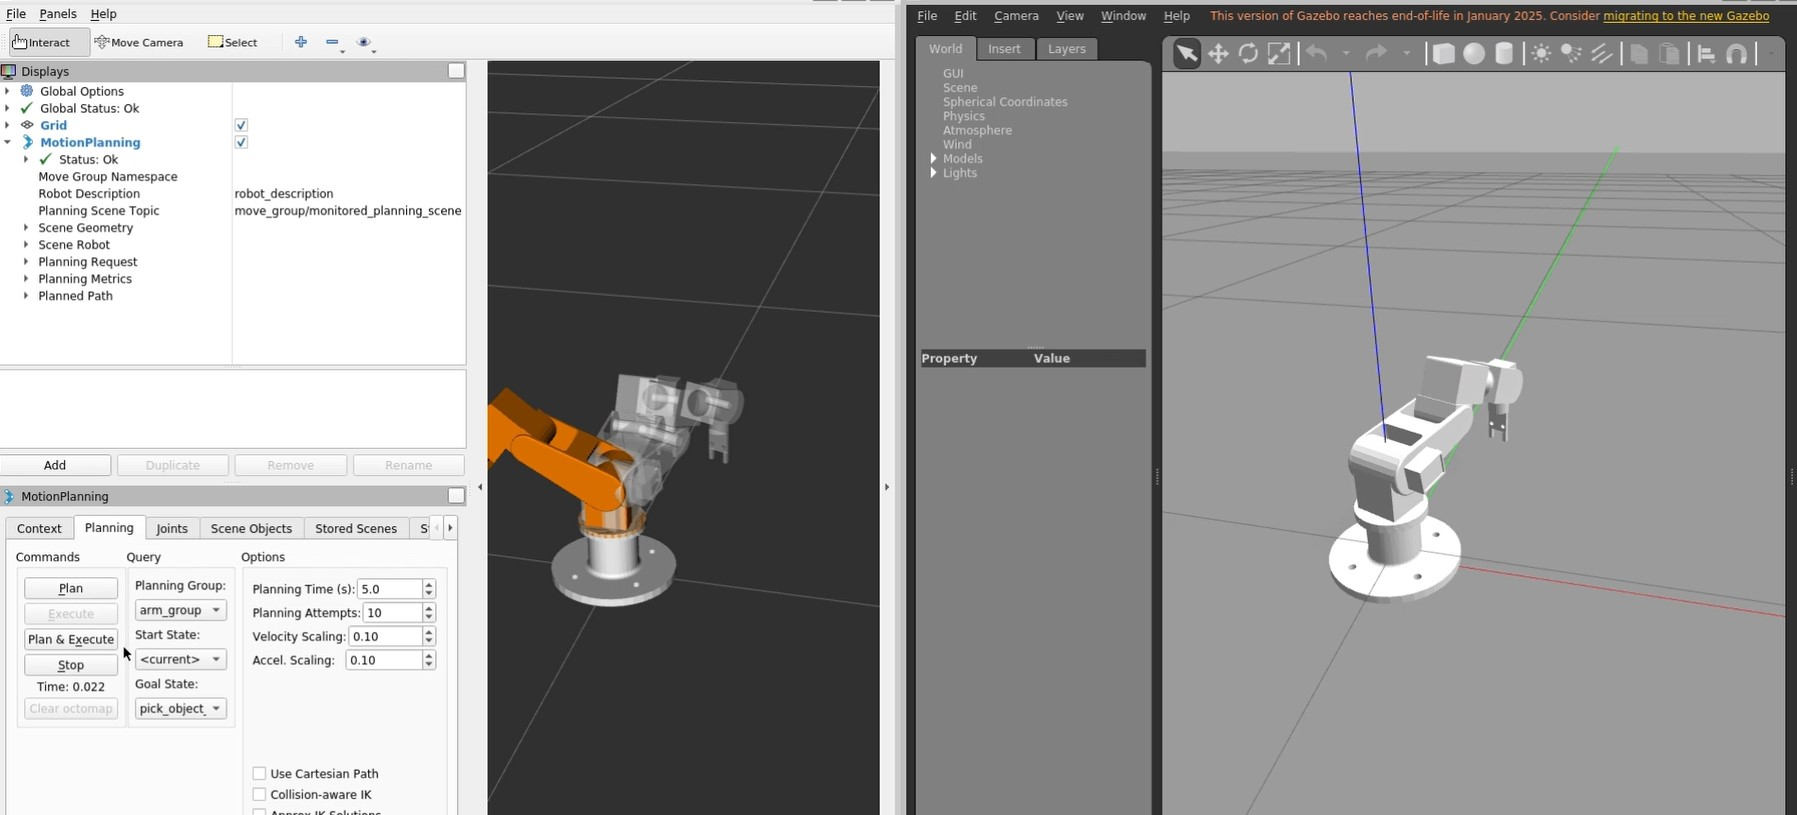
\includegraphics[width=0.8\textwidth]{GazeboRViz.jpg}
	\caption{Visualización del robot en RViz y Gazebo}
	\label{fig:GazeboYrviz}
\end{figure}
